

\section{Desain Interaksi}

Menurut \textcite{PreeceRogersSharp15}, desain interaksi adalah proses mendesain suatu produk yang interaktif untuk menciptakan sebuah pengalaman yang meningkatkan kualitas dari cara kerja, komunikasi, dan interaksi dari pengguna produk. Untuk memberi konteks tentang apa yang didesain, beberapa aspek yang seringkali ditegaskan adalah \textit{user interface} (UI), rekayasa perangkat lunak, \textit{user-centered design}, dan desain produk. Desain interaksi juga dapat dilihat sebagai basis yang fundamental dalam beberapa displin, bidang, dan pendekatan yang berhubungan dengan proses penelitian dan desain sistem berbasis komputer. Maka dari itu, seringkali beberapa aspek dari pendekatan-pendekatan yang memakai pedoman desain interaksi seringkali bertumpang tindih. Preece dkk. mengilustrasikannya pada Gambar \ref{fig:desain_interaksi}.


\begin{figure}[h]
  \centering
  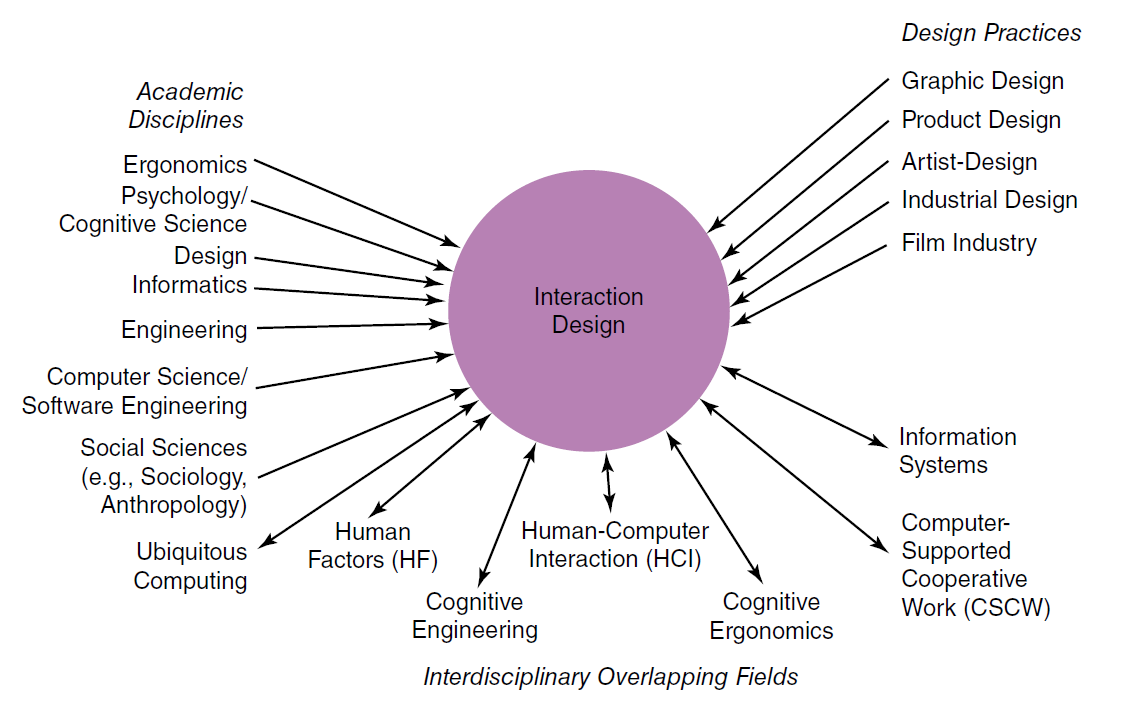
\includegraphics[width=\textwidth]{chapter-2-interaction-design.png}
  \caption{Hubungan studi antardisiplin terkait desain interaksi (Panah dua arah berarti saling tumpang tindih) \textcite{PreeceRogersSharp15}}
  \label{fig:desain_interaksi}
\end{figure}

\FloatBarrier

\subsection{Pendekatan Desain Interaksi}
\label{subsec:pendekatan_id}

Dalam desain interaksi terdapat beberapa pendekatan utama yang dapat digunakan untuk menyusun solusi permasalahan, yaitu \textit{user-centered design} (UCD), \textit{activity-centered design}, \textit{systems design}, dan \textit{genius design} \parencite{saffer2010designing}.

\begin{enumerate}
  \item \textit{User-Centered Design} (UCD)
  \subitem Konsep utama dari UCD adalah mendesain seputar kebutuhan penggunanya. Seorang desainer perlu mendefinisikan tujuan utama dari produk yang dibuat seputar apa yang ingin dicapai oleh penggunanya. Seringkali pengguna pun dilibatkan dalam tahap-tahap pengembangan, seperti pembuatan konsep, pengumpulan data, serta proses pengujian. Hal ini bertujuan untuk menjauhkan produk akhir dari preferensi desainer dan mendekatkan pada preferensi penggunanya sendiri.
   
  \item \textit{Activity-Centered Design}
  \subitem Berbeda dari UCD, pendekatan dengan \textit{activity-centered design} akan memfokuskan seputar kegiatan tertentu. Kegiatan yang dimaksud dapat didefinisikan sebagai kumpulan tugas yang dilakukan untuk mencapai tujuan tertentu. \textit{Activity-centered design} mengharuskan desainer untuk membuat solusi di seputar kegiatan dan menopang kegiatan tersebut, melainkan tujuan dari kegiatan tersebut. Desainer juga harus membedakan maksud dari sebuah aktivitas dengan tujuannya, di mana mereka harus menitikberatkan fokus desain pada maksud dari aktivitas.
 
  \item \textit{Systems Design}
  \subitem \textit{Systems design} adalah pendekatan yang memfokuskan permasalahan pada keseluruhan sebuah sistem dalam proses desainnya. Sistem yang dimaksud bisa terdiri dari banyak komponen pendukung seperti manusia, perangkat keras dan lunak, mesin, dan objek lain sehingga permasalahan yang dihadapi cenderung lebih kompleks.
 
  \item \textit{Genius Design}
  \subitem Pendekatan dengan \textit{Genius Design} mengandalkan sepenuhnya terhadap pengalaman, keahlian, serta preferensi dari desainernya sendiri dalam membuat keputusan desain. Keterlibatan pengguna sangat jarang dan biasanya hanya ada untuk memvalidasi apakah desain yang diprediksi sesuai dengan yang desainer inginkan. Pendekatan ini dinilai memiliki resiko-resiko yang cukup besar namun terkadang dilakukan karena alasan yang lebih kuat daripada resiko tersebut.
 
\end{enumerate}

\subsection{\textit{User-Centered Design} (UCD)}
Seperti yang telah dijelaskan pada subsubbab \ref{subsec:pendekatan_id}, pendekatan UCD memusatkan perhatian proses desain pada pengguna. UCD sendiri merupakan turunan dari cabang ilmu HCI (\textit{Human-Computer Interaction}), yaitu metodologi rekayasa perangkat lunak bagi pengembang yang ditujukan agar perangkat lunak dapat memenuhi kebutuhan penggunanya \parencite{lowdermilk2013user}. Namun pendekatan ini tidak semerta-merta menanyakan langsung keingingan pengguna untuk produknya, karena hal ini dapat membuat produk yang dibuat bias ke pihak tertentu. UCD memiliki tahap dan panduan di mana seorang desainer atau ahli UCD akan mengidentifikasi profil dari penggunanya serta perilaku dan preferensi terhadap aspek-aspek sebuah produk. Informasi yang didapat akan kemudian digunakan dalam proses desain \parencite{10.1145/1621995.1621997}.

Dalam pendekatan UCD, seorang desainer juga tidak hanya membuat desain dengan tampilan antarmuka yang bagus. Desainer harus memastikan agar desain yang dibuatnya menyelesaikan permasalahan awal sesuai dengan riset yang telah dilakukan dan data yang telah diambil dari pengguna. Desainer bertanggung jawab untuk melakukan evaluasi dengan \textit{user} untuk memastikan desain yang telah dibuatnya tepat sasaran \parencite{lowdermilk2013user}.

Dalam penerapannya, pendekatan UCD harus mengikuti prinsip-prinsip tertentu. Menurut \textcite{iso9241-210:2010}, berikut adalah prinsip-prinsip standar yang perlu diikuti

\begin{enumerate}
  \item Desain dibuat berdasarkan pemahaman jelas atas pengguna, tugas-tugas, dan lingkungannya.
  \item Pengguna dilibatkan keseluruhan proses desain dan perkembangannya.
  \item Desain akan diubah dan diperbaiki secara terus-menerus sesuai dengan evaluasi dari pengguna.
  \item Proses UCD dilakukan secara berulang (iteratif).
  \item Desain meliputi keseluruhan \textit{user experience}.
  \item Pembuatan desain melibatkan berbagai perspektif dan kemampuan multidisipliner.
\end{enumerate}

\subsubsection{Proses-Proses dalam UCD}

Dalam melakukan perancangan dengan menerapkan pendekatan UCD, terdapat beberapa standar alur pekerjaan yang dapat diikuti. Salah satu yang umum digunakan adalah alur kerja standar ISO 9241-210. Berikut adalah alur kerja UCD sesuai dengan standar ISO 9241-210 yang tercantum pada Gambar II.2.

Terlihat pada diagram alur kerja pada Gambar \ref{fig:diagram_iso2}, terdapat beberapa kegiatan yang dilakukan secara iteratif. Kegiatan-kegiatan yang dilakukan secara iteratif tersebut merupakan komponen utama dalam kerangka UCD. Berikut adalah penjelasan mengenai kegiatan-kegiatan tersebut:

\begin{figure}[h]
  \centering
  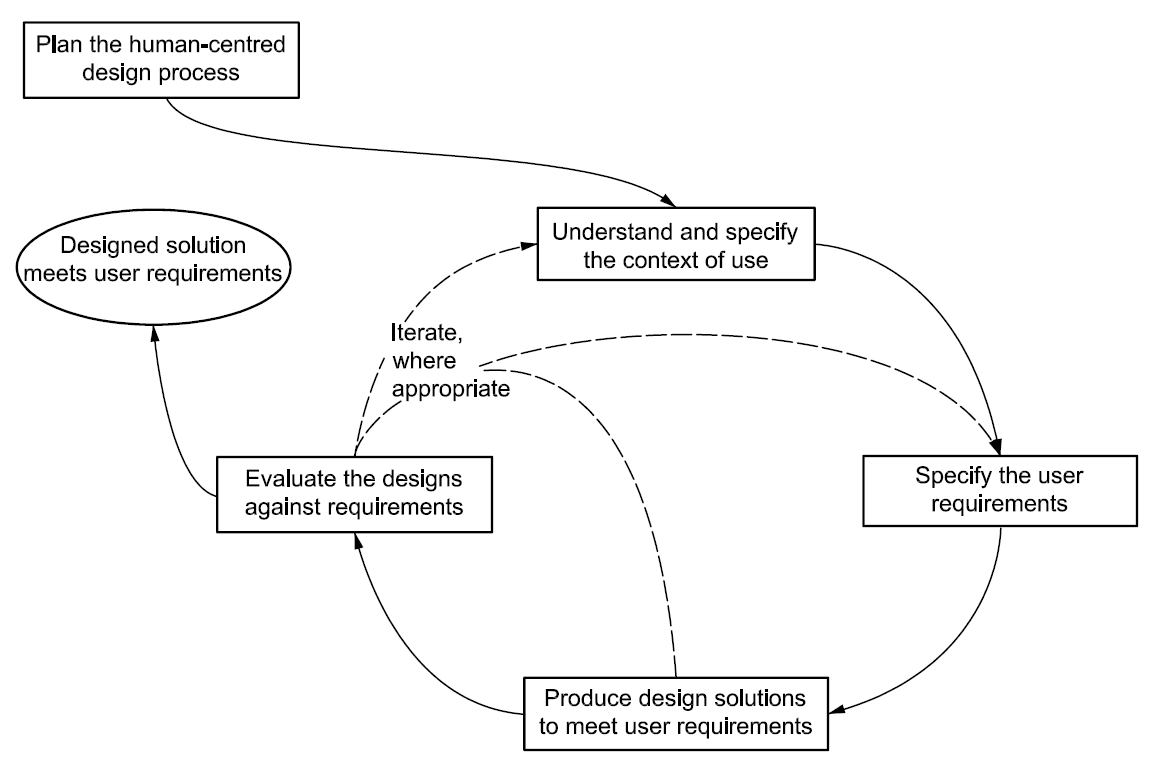
\includegraphics[width=0.9\textwidth]{chapter-2-ucd-figure.png}
  \caption{Alur kerja \textit{User-Centered Design} (\parencite{iso9241-210:2010})}
  \label{fig:diagram_iso2}
\end{figure}
\FloatBarrier

\begin{enumerate}
  \item Memahami dan merincikan konteks penggunaan produk
  \subitem Pada tahap ini dilakukan pengumpulan dan analisa informasi mengenai konteks pemakaian produk. Hal ini bertujuan untuk mengungkapkan adanya kebutuhan, permasalahan, serta batasan dari produk yang penting untuk pengembangan solusi yang akan dibuat. Konteks pemakaian ini perlu mencakup informasi mengenai keseluruhan \textit{stakeholder}, karakteristik target pengguna, tujuan dan kegiatan dari pengguna, serta lingkungan di mana sistem akan dibuat atau dikembangkan. Jika UCD diterapkan pada produk yang sudah dibuat, maka beberapa informasi yang sudah tersedia dapat digunakan untuk melakukan modifikasi atau meningkatkan kualitas produk.
   
  \item Merincikan kebutuhan pengguna
  \subitem Pada tahap ini dilakukan identifikasi dan analisa lebih lanjut terhadap data-data yang telah dikumpulkan pada tahap sebelumnya. Dari hasil analisa akan didapatkan kebutuhan pengguna yang perlu dipenuhi dalam desain yang akan dibuat nanti. Kebutuhan pengguna yang didapat juga perlu mempertimbangkan batasan yang perlu diikuti sesuai dengan konteks pemakaian produk.
  
  \item Membuat solusi desain yang memenuhi kebutuhan pengguna
  \subitem Tahap selanjutnya adalah membuat prototipe desain sesuai dengan kebutuhan pengguna yang telah diidentifikasi pada fase sebelumnya. Prototipe desain yang dimaksud adalah produk implementasi desain aplikasi yang sudah menyerupai produk akhir, tanpa adanya implementasi unsur-unsur teknikal aplikasi tersebut. Hal ini bertujuan agar pengguna dapat memahami interaksi dan antarmuka dari desain aplikasi untuk dievaluasi pada tahap selanjutnya sebelum menjalani implementasi akhir.
  
  \item Mengevaluasi desain yang dibuat terhadap kebutuhan
  \subitem Proses evaluasi adalah proses untuk menentukan apakah desain aplikasi yang dibuat telah menyelesaikan permasalahan atau memenuhi kebutuhan yang diidentifikasi pada tahap-tahap sebelumnya. Proses evaluasi juga dilakukan untuk mengetahui apakah desain aplikasi sesuai dengan \textit{user experience goals} dan \textit{usability goals} yang diharapkan. Proses evaluasi tidak menutup kemungkinan adanya wawasan baru mengenai kebutuhan pengguna atau desain aplikasinya sendiri. Hasil dari evaluasi akan menentukan apakah desain tersebut layak dilanjutkan ke tahap implementasi atau diperlukan iterasi untuk menjalani perbaikan.

\end{enumerate}



\subsection{\textit{Usability Goals} dan \textit{User Experience Goals}}
\label{subsec:goals}
Untuk mendesain produk yang tepat bagi pengguna, seorang desainer perlu mengerti kebutuhan pengguna dengan menentukan tujuan yang jelas dari pengembangan produk interaktif tersebut. \textcite{PreeceRogersSharp15} menyebutkan bahwa untuk mencapainya, tujuan dapat diklasifikasikan sesuai dengan \textit{usability goals} dan \textit{user experience goals}.

% http://bpm.umg.ac.id/aset/images/download/M4-Standar-Rujuka-BA(1-8-2017).pdf


\textit{Usability goals} mengarahkan produk untuk mencapai kriteria \textit{usability} tertentu. \textit{Usability goals} mencakup bagaimana cara untuk mengoptimalisasi interaksi pengguna dengan produk untuk melakukan kegiatannya. \textit{Usability goals} dapat diuraikan menjadi 6 tujuan berikut
\begin{enumerate}
  \item Efektif untuk digunakan (\textit{effectiveness}) adalah tujuan yang menunjukkan apakah suatu produk sukses dalam menjalankan tugasnya.
  \item Efisien untuk digunakan (\textit{efficiency}) adalah tujuan yang menunjukkan bagaimana sebuah produk dapat membantu pengguna dalam mencapai tujuannya. Sebuah produk dapat dikatakan efisien jika penggunanya dapat melakukan suatu kegiatan dalam langkah-langkah yang sederhana dan tidak menuntut pengguna untuk mempelajari langkah-langkah tersebut terlalu lama.
  \item Aman untuk digunakan (\textit{safety}) adalah tujuan yang menunjukkan bagaimana sebuah produk dapat melindungi penggunanya dari situasi yang berbahaya atau tidak diinginkan, atau melakukan hal-hal yang bersifat destruktif. Tujuan ini dapat dicapai dengan meminimalisir resiko yang dapat ditemui pengguna atau memberikan opsi untuk membatalkan aksinya. Tujuan ini juga menunjukkan bagaimana sebuah produk membantu penggunanya mengeksplorasi produk secara percaya diri.
  \item Memiliki utilitas yang baik (\textit{utility}) adalah tujuan yang menunjukkan bagaimana sebuah produk menyediakan fungsionalitas yang baik untuk membantu pengguna melakukan hal yang dibutuhkan atau diinginkan.
  \item Mudah untuk dipelajari (\textit{learnability}) adalah tujuan yang menunjukkan seberapa mudah sebuah produk untuk dipelajari hingga pengguna dapat menggunakannya dengan benar.
  \item Mudah untuk mengingat penggunaan (\textit{memorability}) adalah tujuan yang menunjukkan seberapa mudah bagi pengguna untuk mengingat bagaimana cara menggunakan sebuah produk setelah mempelajarinya.
\end{enumerate}

\textit{User experience goals} lebih bersifat subjektif dibandingkan \textit{usability goals} karena mencakup berbagai jenis emosi dan pengalaman yang dirasakan oleh pengguna saat berinteraksi dengan produk. \textit{User experience goals} juga berhubungan erat dengan estetika dari produk. \textit{User experience goals} terdiri dari 2 jenis, yaitu tujuan yang diharapkan dan tujuan yang tidak diharapkan \parencite{PreeceRogersSharp15}. Pembagiannya dapat dilihat pada Tabel \ref{tab:ux_goals}.

\RaggedLeft
\begin{footnotesize}
\begin{longtable}[c]{|>{\cbnormspacing}m{0.44\textwidth}|>{\cbnormspacing}m{0.49\textwidth}|}
  \caption{\textit{User experience goals} yang diharapkan dan tidak diharapkan}
  \label{tab:ux_goals} \\
  \hline \rowcolor[HTML]{A3E5F5}
  \centering\textbf{\textit{User experience goals} yang diharapkan} & \textbf{\textit{User experience goals} yang tidak diharapkan} \\ \hline \endfirsthead
  \hline \rowcolor[HTML]{A3E5F5}
  \centering\textbf{\textit{User experience goals} yang diharapkan} & \textbf{\textit{User experience goals} yang tidak diharapkan} \\ \hline \endhead
  
  \hline \endfoot
  
  1.	Satisfying              & 1.  Boring                  \\
  2.	Helpful                 & 2.  Unpleasant              \\
  3.	Fun                     & 3.  Frustrating             \\
  4.	Enjoyable               & 4.  Patronizing             \\
  5.	Motivating              & 5.  Making one feel guilty  \\
  6.	Provocative             & 6.  Making one feel stupid  \\
  7.	Engaging                & 7.  Annoying                \\
  8.	Challenging             & 8.  Cutesy                  \\
  9.	Surprising              & 9.  Childish                \\
  10.	Pleasurable             & 10. Gimmicky                \\
  11.	Enhancing sociability   &                             \\
  12.	Rewarding               &                             \\
  13.	Exciting                &                             \\
  14.	Supporting creativity   &                             \\
  15.	Emotionally fulfilling  &                             \\
  16.	Entertaining            &                             \\
  17.	Cognitively stimulating &                             \\
  18.	Experiencing flow       &                             \\
\end{longtable}
\end{footnotesize}
\justifying
\FloatBarrier


\subsection{Prinsip Desain Interaksi}
\label{subsec:prinsip_interaksi}
Prinsip desain interaksi adalah abstraksi umum untuk mengarahkan desainer dalam berpikir dari aspek-aspek yang berbeda dalam mendesain pengalaman pengguna. Prinsip desain dihasilkan dari gabungan antara pengetahuan berteori, pengalaman desainer, dan nalar wajar manusia. Prinsip desain ditujukan untuk membantu desainer dalam menjelaskan dan mengembangkan desain mereka secara konseptual, namun bukan sebagai cara mendesain sebuah antarmuka dari awal. Menurut \textcite{PreeceRogersSharp15}, terdapat banyak prinsip desain yang sudah disetujui secara umum, namun berikut adalah beberapa prinsip paling umum yang berkaitan dengan bagaimana pengguna melihat dan memanfaatkan suatu desain dalam mencapai tujuannya

\begin{enumerate}
  \item \textit{Visibility}
  \subitem Visibilitas dari sebuah fitur mempengaruhi jumlah informasi yang diperlihatkan kepada pengguna. Tingginya tingkat visibilitas akan membantu pengguna dalam menentukan aksi yang dapat dilakukan. Posisi dari fitur terhadap bagaimana fitur tersebut digunakan juga dapat menentukan tingkat kemudahan untuk menggunakan fitur tersebut.
   
  \item \textit{Feedback}
  \subitem \textit{Feedback} atau umpan balik berhubungan dengan prinsip \textit{visibility}. Sebuah aksi layaknya dipasangi dengan sebuah reaksi untuk memberikan pengguna konfirmasi bahwa aksinya berhasil dilakukan atau tidak, membantunya dalam melanjutkan aktivitasnya. Informasi yang dikirimkan sebagai reaksi dapat bersifat taktil, verbal, visual, auditori, atau kombinasinya.
   
  \item \textit{Constraints}
  \subitem Sifat \textit{constraints} menunjuk pada interaksi apa saja yang bisa dilakukan pengguna di saat tersebut, tanpa menghilangkan aksi yang tidak bisa dilakukan. Umumnya, hal ini dapat dicapai dengan menonaktifkan sebuah opsi dalam kelompok pilihan. \textit{Constraints} juga membatasi persepsi pengguna dalam merepresentasikan informasi hanya dengan cara yang diharapkan desainer. Hal ini dapat dicapai dengan menunjukkan relasi yang jelas antarobjek.
   
  \item \textit{Consistency}
  \subitem Konsistensi dalam antarmuka menunjukkan bahwa fitur-fitur dengan elemen yang mirip akan melakukan aksi yang mirip juga atau menghasilkan reaksi yang mirip. Konsistensi akan meningkatkan tingkat kemudahan sebuah fitur untuk dipelajari, dengan cukup mempelajari satu fitur pengguna dapat mengerti fitur lain dengan elemen yang mirip, walaupun tiap fitur memiliki fungsinya sendiri. Contohnya adalah fitur di sebelah tombol \textit{toggle} menunjukkan bahwa pengaturannya bisa dinyalakan / dimatikan.
   
  \item \textit{Affordance}
  \subitem \textit{Affordance} adalah sifat dari objek yang menandakan cara penggunaannya. Contohnya, sebuah \textit{mouse} digunakan dengan ditekan dengan melihat bagaimana tombol \textit{mouse} itu didesain. Semakin tinggi tingkat \textit{affordance} atau semakin jelas bagaimana cara suatu objek digunakan, maka semakin mudah untuk menggunakannya atau belajar menggunakannya.
   
\end{enumerate}

\subsection{Tipe Interaksi}
\label{subsec:tipe_interaksi}

Dalam menyusun konsep desain, penentuan cara pengguna berinteraksi dengan produk / aplikasi akan didasarkan pada tipe interaksi dari desainnya. Menurut \textcite{PreeceRogersSharp15}, ada 5 tipe utama, yaitu \textit{instructing}, \textit{conversing}, \textit{manipulating}, \textit{exploring}, dan \textit{responding}. Menentukan tipe interaksi dari desain dapat membantu untuk menyusun model konseptual sebelum menentukan tipe antarmuka dari desainnya. Suatu sistem tidak terkekang dalam memiliki satu jenis tipe interaksi, pengguna dapat merasakan pengalaman yang berbeda di bagian-bagian sistem dengan tipe interaksinya masing-masing. Berikut adalah penjelasan tentang tipe-tipe interaksi.

\begin{enumerate}
  \item \textit{Instructing}
  \subitem Pada desain yang menerapkan tipe interaksi \textit{instructing} pengguna akan melakukan aktivitasnya dengan cara memberikan instruksi kepada sistem. Pengguna dapat memberikan instruksi dengan mengetikan perintah, memilih opsi dari menu, mengatakan perintahnya ke mikrofon, memberikan gestur, atau sesederhana menekan satu atau kombinasi tombol. Keuntungan dalam memilih tipe interaksi ini adalah kecepatan dan efisiensi interaksi, cocok untuk aksi yang perlu dilakukan berulang kali. Contoh kasus yang menggunakan tipe interaksi \textit{instructing} adalah sebuah \textit{vending machine}, di mana konsumen memilih makanan yang ingin dibeli baik dengan mengetikkan nomor label makanan.

  \item \textit{Conversing}
  \subitem Tipe interaksi \textit{conversing} berdasar pada konsep di mana pengguna akan melakukan percakapan dengan sistem. Sistem didesain untuk membalas pengguna sebagaimana manusia biasa akan menjawab, berbeda dengan tipe interaksi \textit{instructing} di mana sistem hanya menuruti perintah yang diberikan. Pengguna mampu mendapatkan saran, jawaban lebih pribadi, atau berdiskusi dengan sistem. Pada umumnya, sistem akan memanfaatkan teknologi \textit{voice-recognition}, AI, atau teknologi berbasis \textit{natural-language} lainnya dalam menerima input, dan menggunakan pembangkitan suara atau cukup kalimat tertulis untuk memberikan balasan. Tipe interaksi ini dapat ditemukan pada sistem penasehat, fasilitas bantuan, serta \textit{chatbot}.
  
  \item \textit{Manipulating}
  \subitem Tipe interaksi \textit{manipulating} melibatkan tindakan memanipulasi sebuah objek layaknya di dunia nyata, seperti menggerakan (\textit{dragging}), membuka, dan menutup. Pengguna juga dapat melakukan aksi yang mungkin tidak dapat dilakukan di dunia nyata, seperti \textit{stretching}, \textit{shrinking}, memperbesar, dan memperkecil objek. Tujuan yang ingin dicapai adalah untuk memberikan pengguna perasaan senyata mungkin bahwa mereka sedang beinteraksi langsung dengan objek digital. Prinsip dari tipe interaksi ini adalah objek yang ada di layar tetap tampak selama pengguna memanipulasinya, dan memberikan \textit{feedback} yang langsung ketika dimanipulasi untuk mempertahankan perasaan nyatanya. Walaupun tipe interaksi ini dapat membuat pengguna mudah berinteraksi dengan objek, terdapat beberapa aksi yang sebaiknya menggunakan tipe interaksi lain seperti \textit{instructing}. Contohnya adalah ketika memperbaiki \textit{typo} yang berulang di suatu dokumen, melainkan mengubahnya dengan mencari dan menggantinya satu per satu, lebih baik untuk memberikan instruksi kepada sistem untuk mencari \textit{typo} tersebut di seluruh dokumen dan langsung mengganti semuanya.
  
  \item \textit{Exploring}
  \subitem Sistem yang menggunakan tipe interaksi \textit{exploring} melibatkan penggunanya untuk bergerak di sebuah lingkungan baik virtual maupun fisik. Lingkungan sistem dapat mendeteksi ketika pengguna melakukan aksi tertentu dan memicu suatu peristiwa yang dapat dirasakan dan diinteraksi oleh pengguna. Lingkungan sistem tidak selalu harus berbentuk dunia virtual 3D, tetapi kebanyakan sistem yang mengadopsi tipe interaksi \textit{exploring} memilikinya, seperti eksibisi virtual yang diakses menggunakan perangkat VR atau sebuah \textit{game}.
  
  \item \textit{Responding}
  \subitem Sistem dengan tipe interaksi \textit{responding} akan menginisiasi interaksinya dengan memberikan, menunjukkan, atau mendeskripsikan sesuatu kepada pengguna, dan menunggu sebuah tanggapan. Interaksi yang diberikan sistem bergantung pada konteks yang sedang dialami pengguna atau dideteksi sistem.  Contohnya sebuah aplikasi dapat memberikan rekomendasi restoran yang berada di dekat pengguna ketika melewati suatu jalan, atau sebuah \textit{smartwatch} memberi notifikasi bahwa penggunanya sudah berhasil berjalan sebanyak 10.000 langkah. Tantangan desain yang menggunakan tipe interaksi ini adalah mengetahui kapan pengguna merasa informasi yang diberikan akan merasa berguna, dan menghindari interaksi yang dirasa dapat mengganggu pengguna.

\end{enumerate}
